\documentclass[UTF8,a4paper,11pt,fontset=none]{ctexart}
\usepackage[margin=2.15cm]{geometry}
\usepackage{amsmath,amssymb}
\usepackage{booktabs,longtable,array}
\usepackage{graphicx}
\usepackage{float}
\usepackage{caption}
\usepackage{enumitem}
\usepackage{xcolor}
\usepackage{hyperref}
\setmainfont{DejaVu Serif}
\setsansfont{DejaVu Sans}
\setmonofont{DejaVu Sans Mono}
\setCJKmainfont{Droid Sans Fallback}
\setCJKsansfont{Droid Sans Fallback}
\setCJKmonofont{WenQuanYi Zen Hei Mono}
\hypersetup{colorlinks=true,linkcolor=blue!45!black,urlcolor=blue!60!black,citecolor=blue!45!black,
  pdftitle={GUI Grounding 复现、外推与粗细粒度视觉搜索技术报告},pdfauthor={GUI Grounding 实验复现与扩展}}
\captionsetup{font=small,labelfont=bf}
\setlist{itemsep=2pt,topsep=4pt}
\linespread{1.12}
\newcommand{\pp}{\ensuremath{\,\mathrm{pp}}}
\newcommand{\code}[1]{\texttt{#1}}

\title{\bfseries 从槽位读数到粗细粒度视觉搜索\\GUI Grounding 复现、外推与算法实验技术报告}
\author{GUI Grounding 实验复现与扩展}
\date{2026 年 11 月}

\begin{document}
\maketitle

\begin{abstract}
本报告系统整理 GUI-Decisions 槽位读数方法的复现、自然图像外推及高分辨率 GUI grounding 改进实验。所有新增测量均基于 GUI-Decisions-2B 和本地 CPU 推理，不使用远程推理服务。原始 ScreenSpot 全量点命中率为 76.49\%，与文章报告值一致；RefCOCO 随机目标零样本点命中率达到 91.41\%，但小目标降至 75.78\%。在更困难的 ScreenSpot-Pro 上，全图槽位读数仅为 13.41\%。一次 512px 固定裁剪重读将其提升至 40.73\%；通过严格的校准集/留出集协议，进一步确定的 768px 裁剪与 KDE-grid 局部读出组合达到 47.88\%，留出集为 48.42\%。结果说明：槽位读数有效消除了坐标文本解码，但高分辨率场景的主要误差同时来自二维分布读出与视觉分辨率损失；简单的粗细粒度视觉搜索比复杂门控更稳定。图标目标仍只有 20.00\%，是当前最主要的短板。
\end{abstract}

\section{研究目标与结论摘要}
本文回答四个问题：（1）文章的槽位读数结果能否在本地复现；（2）该接口能否零样本外推到自然图像指代表达定位；（3）在高分辨率、密集专业 GUI 上，误差主要来自坐标读出还是视觉输入；（4）能否在不重新训练的情况下提高准确率，并量化额外计算成本。

主要结论如下。
\begin{itemize}
  \item \textbf{复现成立。} ScreenSpot 全量 default 读数为 76.49\%（973/1272），接近文章的 77.0\%及模型卡本地值 76.3\%。
  \item \textbf{零样本迁移成立，但不是普遍解决。} RefCOCO 点定位显著优于 vanilla，小目标明显下降；该协议不同于文章附录的框 IoU，不能直接比较。
  \item \textbf{高分辨率下，二次裁剪是最强改进。} ScreenSpot-Pro 全量从 13.41\%提升至 40.73\%（512px default），再到 47.88\%（768px KDE-grid）。
  \item \textbf{KDE 有独立价值，但不能替代局部视觉重读。} 全图 KDE-grid 无额外模型前向提升 4.55 个百分点；局部 KDE-grid 与 768px 裁剪结合后收益更大。
  \item \textbf{不确定样本门控并非普遍有效。} ScreenSpot-Pro 上 1576/1581 个样本仍被判定需要裁剪，几乎不节省计算；全分布方差驱动的自适应窗口也不如固定窗口。
\end{itemize}

\begin{figure}[H]
  \centering
  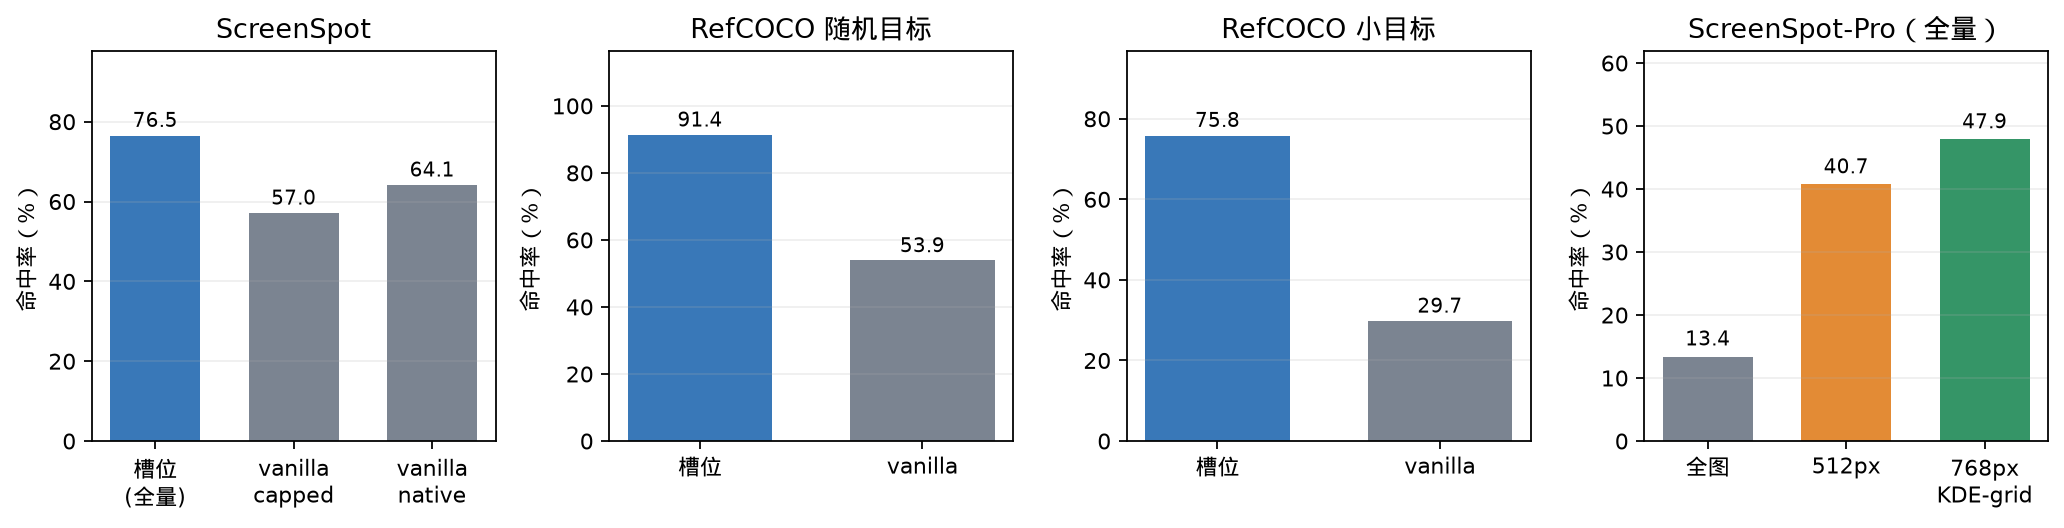
\includegraphics[width=\textwidth]{figures/overview_accuracy.png}
  \caption{核心结果概览。ScreenSpot 的 vanilla 与配对槽位比较使用同一 128 条子集，槽位全量柱仅作背景；RefCOCO 为 128 条；ScreenSpot-Pro 三种方法均为全量 1581 条。}
  \label{fig:overview}
\end{figure}

\section{实验设置}
\subsection{模型、数据与运行环境}
基础代码为官方 \code{infinitylogesh/gui-decisions} 的提交 \code{4afc7f2}，实验脚本和数据分析在工作区中新增。主要模型为 \code{infinitylogesh/GUI-Decisions-2B}（快照 \code{c2cedfd}），vanilla 对照为 \code{mPLUG/GUI-Owl-1.5-2B-Instruct}（快照 \code{528ceae}）。

\begin{table}[H]
\centering\small
\caption{数据集与用途}
\begin{tabular}{>{\raggedright\arraybackslash}p{3.0cm}>{\raggedright\arraybackslash}p{2.0cm}>{\raggedright\arraybackslash}p{8.8cm}}
\toprule
数据集 & 样本量 & 协议与用途 \\
\midrule
ScreenSpot & 1272 & 原始点击框内命中率，全量复现；vanilla 使用 \code{id \% 10 == 0} 的 128 条配对子集。 \\
RefCOCO val & 8415 个去重目标 & 按 COCO 图像 ID 与框去重，XYWH 转 XYXY 并裁剪到 $[0,1]$；每个目标取 \code{answer[0]}，提示为'click + expression'。 \\
RefCOCO 小目标 & 170 个候选，抽样 128 & 面积 $<0.05$；全集中最小面积仍约为 0.0305，不能代表极小物体。 \\
ScreenSpot-Pro & 1581 & 高分辨率专业软件、完整屏幕；点落入 GT 框计为正确。覆盖 23 个应用、6 个类别及文本/图标目标。 \\
\bottomrule
\end{tabular}
\end{table}

所有实验使用 CPU，环境为 Python 3.12、PyTorch 2.15、Transformers 5.22.1，线程设置为 \code{OMP\_NUM\_THREADS=96} 和 \code{MKL\_NUM\_THREADS=96}。模型图像上限保持训练配置（GUI-Owl 为 1MP）；局部裁剪从原图取得，再经过相同处理器。报告中的延迟均为本地 CPU 中位数，\textbf{不能用于验证文章的 RTX PRO 6000 GPU 加速比}。

\subsection{指标与统计方法}
主要指标是点落入 GT 框的比例（Hit@1）。RefCOCO 另报告中心接近率：预测点与框中心在两个归一化轴上的距离均不超过 0.1；中心距离为归一化欧氏距离中位数。配对提升使用 10000 次 paired bootstrap 的 95\%区间，二元命中差异使用双侧精确 McNemar 检验。解析失败计为错误；延迟包含相应模型前向，不把未执行的读取计入。

ScreenSpot-Pro 的算法选择严格划分为前 790 条校准样本与后 791 条留出样本（源样本已用 seed 0 随机打乱）。尺寸与局部读出仅在校准集选择，留出集只执行预选组合；已有 512px default 作为配对参照。

\section{槽位读数与分布近似}
槽位方法在每个答案位置直接读取下一 token 分布，不生成 JSON 坐标。每个轴离散为 256 个 bin。default 读取最大 bin 并用相邻 $\pm2$ 个 bin 做概率加权；peak 仅取最大 bin；expected 取全分布期望。

对空间搜索，实验额外考察独立轴外积近似：
\begin{equation}
  q_{ij}=p_x(i)p_y(j),
\end{equation}
其中 $q_{ij}$ 只是二维联合分布的近似，并非模型直接输出的联合概率。region voting 将空间划为 $16\times16$ 区域并选择最大概率质量区域；sampled KDE 从两个轴独立采样 64 个点并选取核密度峰；KDE-grid 在外积网格上用带宽 0.03 的二维 Gaussian 平滑，再在峰值邻域加权读出。该近似可能把真实的两个二维模态扩展为四个组合，因此其收益必须实测。

\section{原始 ScreenSpot 复现}
\subsection{全量槽位结果}
\begin{table}[H]
\centering\small
\caption{ScreenSpot 全量结果（$n=1272$）}
\begin{tabular}{lcccc}
\toprule
读出 & 命中数 & 命中率 & Wilson 95\%区间 & click 动作准确率 \\
\midrule
default & 973 & \textbf{76.49\%} & [74.09\%, 78.74\%] & 93.79\% \\
peak & 968 & 76.10\% & [73.68\%, 78.36\%] & 93.79\% \\
expected & 754 & 59.28\% & [56.55\%, 61.94\%] & 93.79\% \\
\bottomrule
\end{tabular}
\end{table}

default 与 peak 接近，说明局邻域加权只有小幅影响；expected 显著较差，表明坐标分布存在多峰或长尾，期望会落到候选之间。文章报告值为 77.0\%，模型卡本地值为 76.3\%，本结果处于合理复现范围。

\subsection{vanilla 配对对照}
\begin{table}[H]
\centering\small
\caption{同一 128 条 ScreenSpot 子集的配对比较}
\begin{tabular}{lccc}
\toprule
方法 & 命中率 & 槽位相对提升 & McNemar $p$ \\
\midrule
槽位 default & 78.12\% & --- & --- \\
vanilla，相同 capped 图像 & 57.03\% & +21.09\pp & $1.43\times10^{-5}$ \\
vanilla，native 图像 & 64.06\% & +14.06\pp & 0.00510 \\
\bottomrule
\end{tabular}
\end{table}

CPU 中位延迟分别为：vanilla capped 5.76s、native 11.08s；槽位全量运行时约 1.52s。vanilla 使用原文 agent/tool-call 提示词，\textbf{不是 GUI-Owl 专用 grounding 提示词}，因此该对照证明的是相同 agent 协议下的差异，不是所有提示词条件下的最优公平排名。

\section{自然图像零样本外推}
\subsection{随机目标}
\begin{table}[H]
\centering\small
\caption{RefCOCO 随机 128 个目标（seed 0）}
\begin{tabular}{lccc}
\toprule
方法 & 框内命中率 & 中心接近率 & 中心距离中位数 \\
\midrule
槽位 default / peak & \textbf{91.41\%} & 53.91\% / 54.69\% & 0.1012 / 0.1010 \\
槽位 expected & 85.94\% & \textbf{72.66\%} & \textbf{0.0765} \\
vanilla & 53.91\% & 40.63\% & 0.1505 \\
\bottomrule
\end{tabular}
\end{table}

default 相对 vanilla 提升 37.50 个百分点，paired bootstrap 95\% CI 为 $[28.12,46.88]$；仅槽位正确 51 条、仅 vanilla 正确 3 条，McNemar $p=2.92\times10^{-12}$。vanilla 有 4 条解析失败，生成长度中位数为 52 tokens。seed 1 的独立 128 条复核中，default 仍为 91.41\%，expected 为 86.72\%；两组 default 合计 234/256。

default 更适合'落入框内'，expected 的中心估计反而更好。这提示评估指标会改变最佳读出：若目标是框内命中，尖锐模态更有利；若目标是回归中心，期望可能更平滑。

\subsection{小目标压力测试}
\begin{table}[H]
\centering\small
\caption{RefCOCO 面积 $<0.05$ 的 128 个目标（seed 0）}
\begin{tabular}{lccc}
\toprule
方法 & 框内命中率 & 中心接近率 & 中心距离中位数 \\
\midrule
槽位 default / peak & \textbf{75.78\%} & 64.84\% & 0.0615 \\
槽位 expected & 60.16\% & 63.28\% & 0.0862 \\
vanilla & 29.69\% & 30.47\% & 0.2281 \\
\bottomrule
\end{tabular}
\end{table}

default 相对 vanilla 提升 46.09 个百分点，95\% CI $[36.72,55.47]$，分歧为 63/4 条，$p=1.11\times10^{-14}$。但槽位自身从随机集合的 91.41\%降至 75.78\%，证明小目标仍是明显弱点。典型失败包括复杂关系、位置限定和视觉上不显著的目标。

\section{ScreenSpot-Pro：高分辨率 GUI 改进}
\subsection{全图分布读出与固定裁剪}
ScreenSpot-Pro 的目标平均仅占图像约 0.07\%，原始 ScreenSpot 约为 2.01\%\cite{screenspotpro}。全量 1581 条结果如下。
\begin{table}[H]
\centering\small
\caption{ScreenSpot-Pro 全图读出与 512px 固定裁剪（全量 $n=1581$）}
\begin{tabular}{lccc}
\toprule
方法 & 命中率 & 相对 default & 额外模型前向 \\
\midrule
default & 13.41\% & --- & 0 \\
peak & 13.22\% & -0.19\pp & 0 \\
expected & 6.58\% & -6.83\pp & 0 \\
region voting & 13.85\% & +0.44\pp，不显著 & 0 \\
sampled KDE & 17.58\% & +4.17\pp & 0 \\
KDE-grid & 17.96\% & +4.55\pp & 0 \\
512px 固定裁剪重读 & \textbf{40.73\%} & \textbf{+27.32\pp} & 1 次 \\
\bottomrule
\end{tabular}
\end{table}

512px 固定裁剪修复 473 条、回退 41 条，提升的 paired bootstrap 95\% CI 为 $[24.92,29.79]$ 个百分点，McNemar $p=3.34\times10^{-94}$。KDE-grid 也有显著但较小的收益：95\% CI $[2.78,6.33]$，$p=4.48\times10^{-7}$。这说明分布读出和视觉分辨率是两个可分离的误差来源。

\subsection{自适应窗口与门控的失败}
在 128 条跨应用随机样本上，default 居中的固定 512px 裁剪为 35.94\%，基于全分布方差的自适应窗口仅为 17.97\%。长尾方差会扩大窗口，使局部放大退化为近似全图重读。KDE 居中固定裁剪为 39.06\%，相比 default 居中的提升不显著（$p=0.48$），且回退更多，因此未用于全量。

全图置信度对正确性的留出 AUROC 为 0.802，但最终门控仍触发 1576/1581 次裁剪。换言之，该模型在 ScreenSpot-Pro 上几乎普遍不确定，门控不能带来实际的延迟节省。接受策略分析还表明，执行第二次读取和采用第二次预测必须分别计费和统计。

\begin{figure}[H]
  \centering
  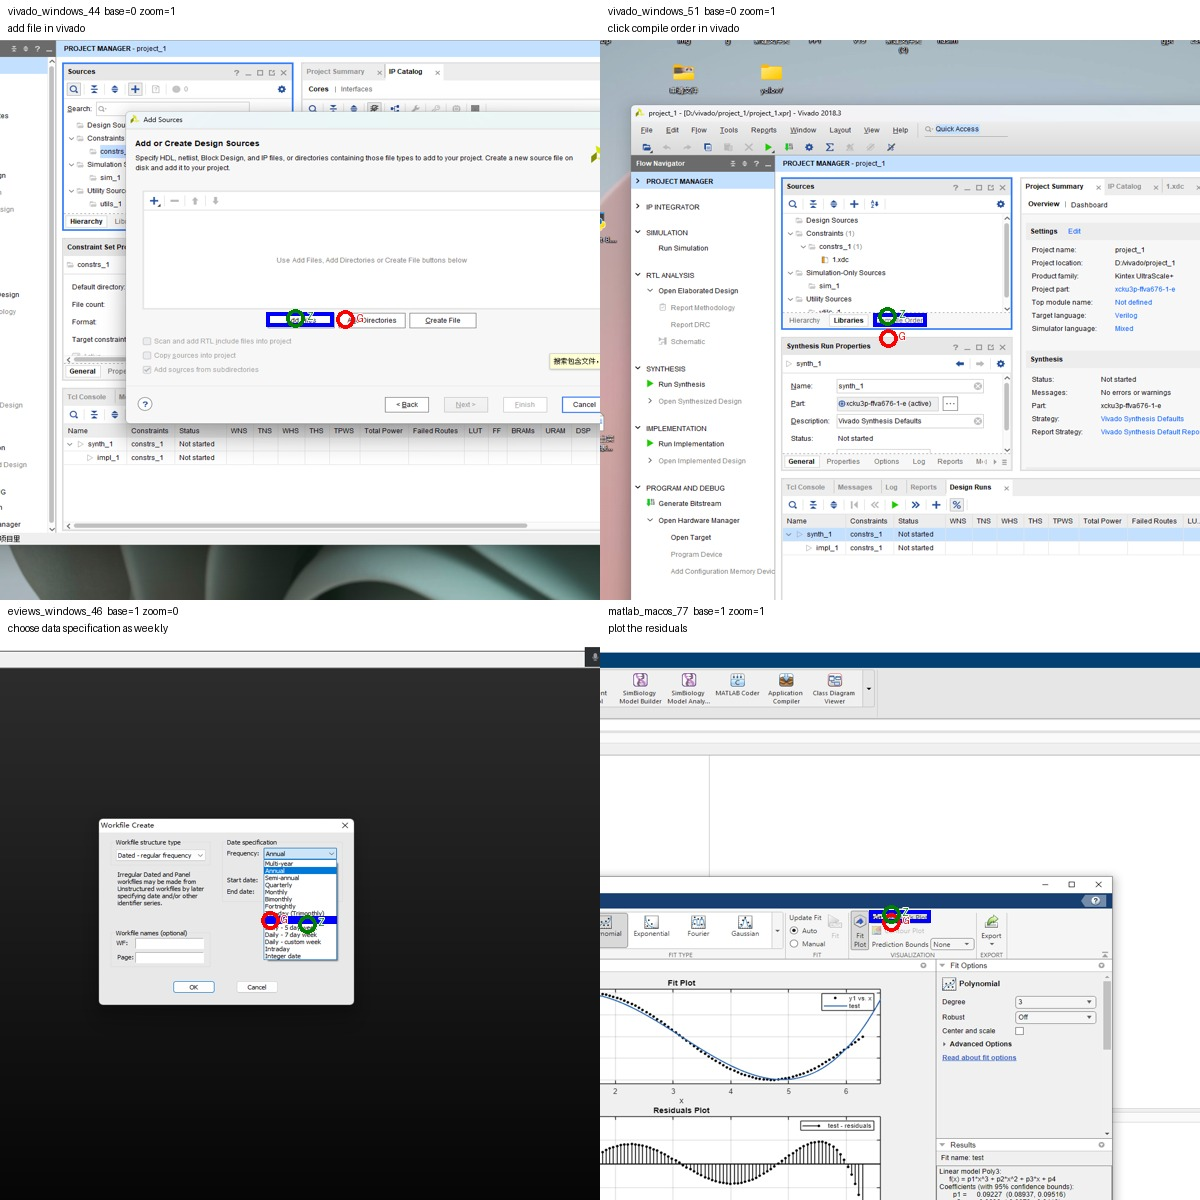
\includegraphics[width=0.92\textwidth]{figures/sspro_zoom_examples.jpg}
  \caption{预测与标注图像抽查。蓝框为 GT，红点 G 为全图结果，绿点 Z 为裁剪结果。上排展示修复，左下展示一次回退，右下为保持正确。坐标映射与标注对齐。}
  \label{fig:examples}
\end{figure}

\section{裁剪尺寸与局部读出消融}
\subsection{校准集选择}
在前 790 条校准样本上扫描五种方形窗口及四种局部读出。图\ref{fig:sweep}显示，KDE-grid 在所有尺寸上均优于 default，768px 达到峰值，1024px 开始下降。
\begin{figure}[H]
  \centering
  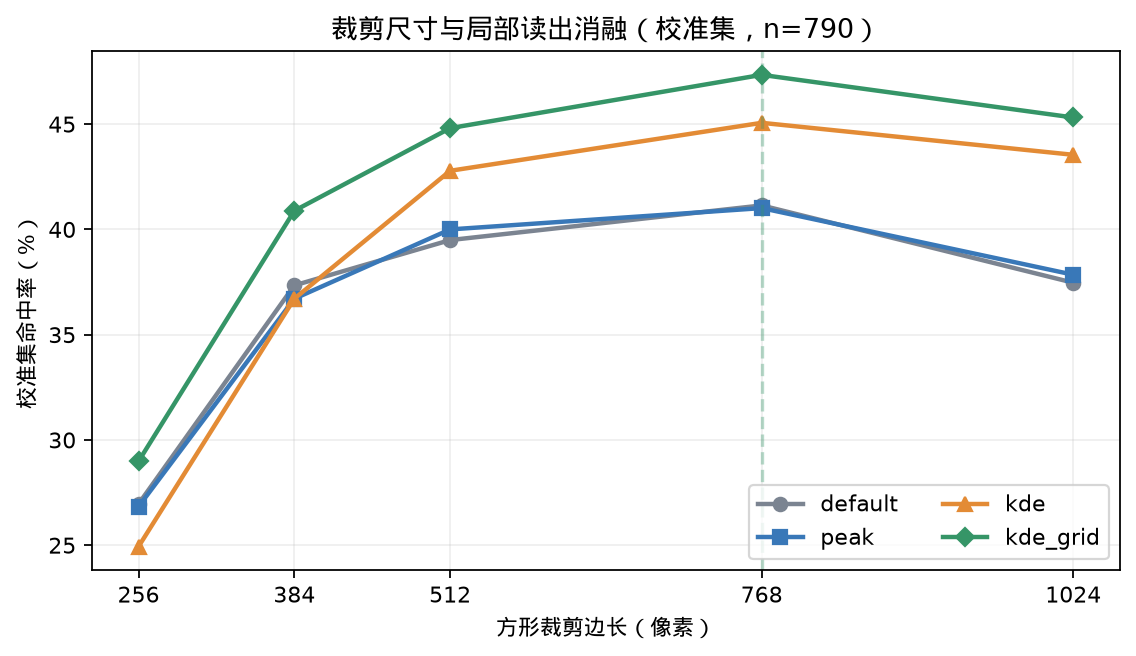
\includegraphics[width=0.78\textwidth]{figures/crop_sweep.png}
  \caption{裁剪尺寸和局部读出消融。选择过程只使用校准集。}
  \label{fig:sweep}
\end{figure}

相同 512px 下，局部 default 为 39.49\%，局部 KDE-grid 为 44.81\%，直接提升 5.32 个百分点，95\% CI $[3.42,7.34]$，$p=1.01\times10^{-7}$。768px KDE-grid 相比 512px KDE-grid 再提高 2.53 点，但校准集内 $p=0.0747$，因此尺寸收益必须依赖留出集确认。

\subsection{留出集与合并结果}
留出集只执行预选的 768px KDE-grid。
\begin{table}[H]
\centering\small
\caption{预选组合的留出验证与全量合并结果}
\begin{tabular}{lccc}
\toprule
方法 & 留出集（$n=791$） & 合并（$n=1581$） & CPU 中位延迟 \\
\midrule
全图 default & 13.91\% & 13.41\% & 约 1.44s \\
512px default & 41.97\% & 40.73\% & 约 1.91s \\
\textbf{768px KDE-grid} & \textbf{48.42\%} & \textbf{47.88\%} & 约 2.38s \\
\bottomrule
\end{tabular}
\end{table}

留出集上，预选组合相比 512px default 提升 6.45 个百分点，95\% CI $[3.67,9.23]$，$p=8.29\times10^{-6}$；90 条由错转对，39 条由对转错。合并后相对 512px default 提升 7.15 点，95\% CI $[5.12,9.17]$，$p=7.33\times10^{-12}$；相对全图提升 34.47 点，757/1581 个样本正确。

延迟增加约 25\%（相对于 512px default 的 CPU 中位延迟），换取 7.15 个百分点的全量准确率提升。KDE 后处理不增加模型前向，主要成本来自更大局部图像的读取。

\begin{figure}[H]
  \centering
  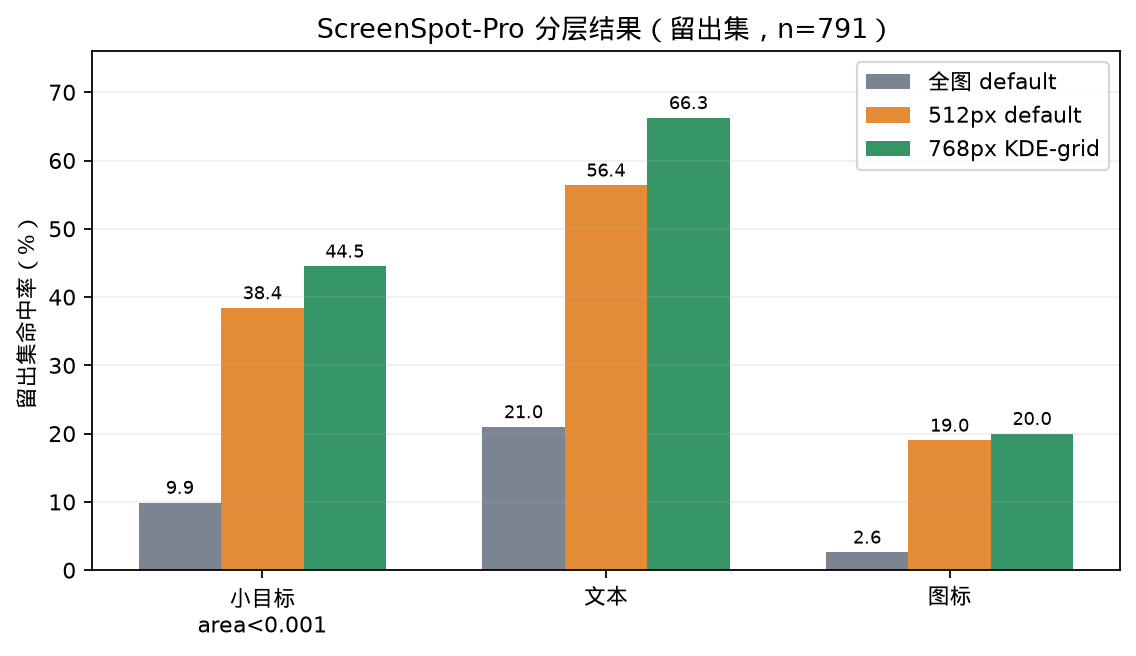
\includegraphics[width=0.78\textwidth]{figures/sspro_breakdown.png}
  \caption{留出集分层结果。文本和小目标受益显著，图标改善有限。}
  \label{fig:breakdown}
\end{figure}

留出集小目标（面积 $<0.001$）从 9.91\%提升至 38.41\%（512px default），再到 44.51\%（768px KDE-grid）；文本从 20.99\%提升至 56.38\%和 66.26\%；图标仅从 2.62\%提升至 19.02\%和 20.00\%。因此后续算法应把图标语义与相似候选区分作为独立问题，而不能只继续放大图像。

\section{讨论}
\subsection{证据链与算法含义}
实验形成了较清晰的递进关系：
\begin{enumerate}
  \item \textbf{读出接口有效：} 槽位可以在不生成坐标文本的情况下保持 ScreenSpot 精度，并零样本迁移到自然图像点定位。
  \item \textbf{独立轴分布不是完整空间表示：} expected 和 region voting 表现较差，KDE 的小幅收益说明多模态确实存在，但独立轴外积无法完整表达二维区域。
  \item \textbf{高分辨率视觉证据是主要瓶颈：} 一次固定裁剪带来的收益远大于任何全图读出后处理。
  \item \textbf{局部视觉与局部分布读出可组合：} 768px 提供合适的上下文与有效分辨率，KDE-grid 进一步修正局部候选选择。
  \item \textbf{复杂搜索并不必然更好：} 全分布方差窗口、KDE 居中和不确定门控均未稳定超过简单固定裁剪。
\end{enumerate}

这些结果与 GUI-Actor、GUI-AIMA 的二维区域监督方向\cite{guiactor,guiaima}、UI-Zoomer 的不确定性搜索\cite{uizoomer}以及 Seg2Click 的子 token 区域预测\cite{seg2click}相互呼应。本文没有复现这些模型的训练结果，相关文献仅用于解释后续研究方向。

\subsection{局限性}
\begin{itemize}
  \item 仅实测 2B 模型；31B、其他 backbone、训练型二维 head 和强化学习未验证。
  \item vanilla 使用 agent/tool-call 提示词，不是专用 grounding 提示词；不能据此声称所有公平提示条件下槽位都优于 vanilla。
  \item 原始 ScreenSpot 与 ScreenSpot-v2 的标注不同，本文不将 76.49\%与近期 v2 分数直接比较。
  \item RefCOCO 使用新的点定位协议，不能与文章附录的 box IoU 直接比较；小目标集合也不代表极小物体。
  \item 128 条 pilot 仅用于探索；核心全量结论以 ScreenSpot-Pro 1581 条及独立留出验证为准。
  \item 延迟全部来自 CPU，未验证 vLLM/SGLang、GPU 并发、prefix cache 或文章所述 NVFP4 服务性能。
  \item Hit@1 不等于在线 agent 任务成功率；尚未执行 OSWorld/WebArena 端到端验证。
  \item $p_xp_y$ 是联合分布近似。要彻底解决二维歧义，需要联合 heatmap、区域 head 或子 token mask，而非继续调 KDE 参数。
\end{itemize}

\subsection{后续实验建议}
短期应以 768px KDE-grid 作为新基线，增加图标/文本、目标面积和应用类别的困难分层，并验证二次局部放大与视图一致性训练。中期应比较三种同数据、同 backbone 输出头：独立 x/y bins、二维 patch heatmap、子 token mask。训练目标可引入背景抑制、尺寸自适应 Gaussian 或 BCE+Dice。长期需在统一 GPU 服务上测量端到端延迟，并在 OSWorld/WebArena 验证在线收益。

\section{可复现性与实验产物}
原始结果保存在 \path{results/}，核心文件包括：
\begin{itemize}
  \item \path{local_gui-decisions-2b_click_0.json}：ScreenSpot 全量复现。
  \item \path{gui-owl-vanilla-s0of10_click_128.json}：vanilla 配对对照。
  \item \path{refcoco-slots-s0_refcoco_point_128.json} 及对应 vanilla、seed 1 和 small 文件：自然图像外推。
  \item \path{zoom-sspro-full-default-s0_screenspot-pro_zoom_1581.json}：ScreenSpot-Pro 全图与 512px 全量结果。
  \item \path{crop-sweep-calibration-s0_790.json}：尺寸与局部读出校准扫描。
  \item \path{crop-heldout-768-kdegrid-s0_791.json}：预选组合留出验证。
  \item \path{crop-sweep-final-s0.json}：校准、留出和合并统计分析。
\end{itemize}

主要实现为 \path{slotread/zoom.py}、\path{scripts/check_zoom_local.py}、\path{scripts/check_crop_sweep_local.py}、\path{scripts/analyze_zoom.py} 和 \path{scripts/analyze_crop_sweep.py}。报告图表由 \path{scripts/generate_report_figures.py} 从原始 JSON 重新生成。实验已通过结果完整性检查、坐标/分布冒烟测试、\code{compileall}、\code{git diff --check} 和 \code{uv build}。

\begin{thebibliography}{9}\small
\bibitem{guidecisions}
Umapathi, Logesh Kumar. \emph{GUI-Decisions: Stop Decoding Coordinates for 3x Faster Computer-Use Grounding}. 2026.
\url{https://huggingface.co/blog/infinitylogesh/gui-decisions-stop-decoding-coordinates}

\bibitem{screenspotpro}
Li, Kaixin et al. \emph{ScreenSpot-Pro: GUI Grounding for Professional High-Resolution Computer Use}. 2025.
\url{https://arxiv.org/abs/2504.07981}

\bibitem{refcoco}
\emph{RefCOCO evaluation data, lmms-lab-encoder/RefCOCO}.
\url{https://huggingface.co/datasets/lmms-lab-encoder/RefCOCO}

\bibitem{guiactor}
Wu et al. \emph{GUI-Actor: Coordinate-Free Visual Grounding for GUI Agents}. NeurIPS 2025.
\url{https://arxiv.org/abs/2506.03143}

\bibitem{guiaima}
Zhou et al. \emph{GUI-AIMA: Coordinate-Free GUI Grounding via Intrinsic Multimodal Attention}. 2026.
\url{https://arxiv.org/abs/2511.00810}

\bibitem{uizoomer}
Chen et al. \emph{UI-Zoomer: Training-Free Adaptive Zoom-In for GUI Grounding}. 2026.
\url{https://arxiv.org/abs/2604.14113}

\bibitem{seg2click}
Huang et al. \emph{Seg2Click: Executable-Region Prediction for GUI Grounding}. 2026.
\url{https://arxiv.org/abs/2610.16234}

\bibitem{relavis}
\emph{ReLaViS: Recurrent Latent Visual Search for GUI Grounding}. 2026.
\url{https://arxiv.org/abs/2610.05185}
\end{thebibliography}

\end{document}
